\item \textbf{{[}YIJC/PRELIM/9569/2021/P2/Q3{]} }

Shoppe e-Commerce has a mobile application for customers to make purchases
through its online platform. All the customers\textquoteright{} details,
product data and ordering records are kept in the database \texttt{shoppe.db}. 

\subsubsection*{Task 3.1 }

Write program code for the webpage \texttt{index.html} for the customer
to log in to their account. The \texttt{/login} route in the server
code should verify the customer\textquoteright s username and password
using the data in the \texttt{Account} table in the database. 
\noindent \begin{center}
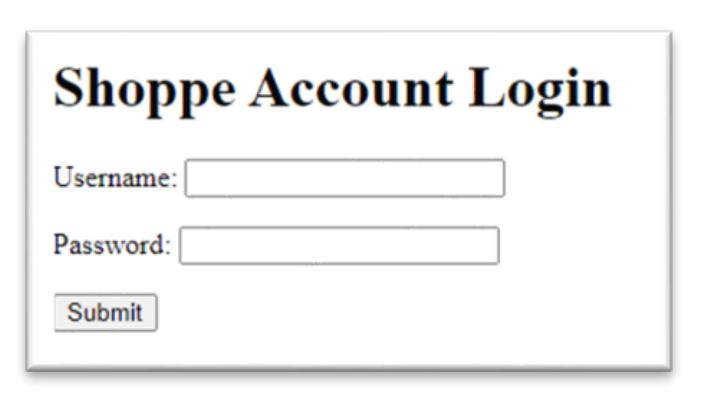
\includegraphics[scale=0.5]{C:/Users/Admin/Desktop/Github/question_bank/LyX/static/img/9569-YIJC-2021-P2-Q3-1}
\par\end{center}

If the log-in details are valid, the customer will receive the webpage
\texttt{display.html}. Otherwise, the customer will be redirected
back to the log-in page. \hfill{} {[}7{]}

\subsubsection*{Task 3.2 }

Write program code for the webpage \texttt{display.html }to display
the customer\textquoteright s details, with the profile picture, and
a menu for the customer to choose the option to update the profile
picture or to check the shopping cart. 
\noindent \begin{center}
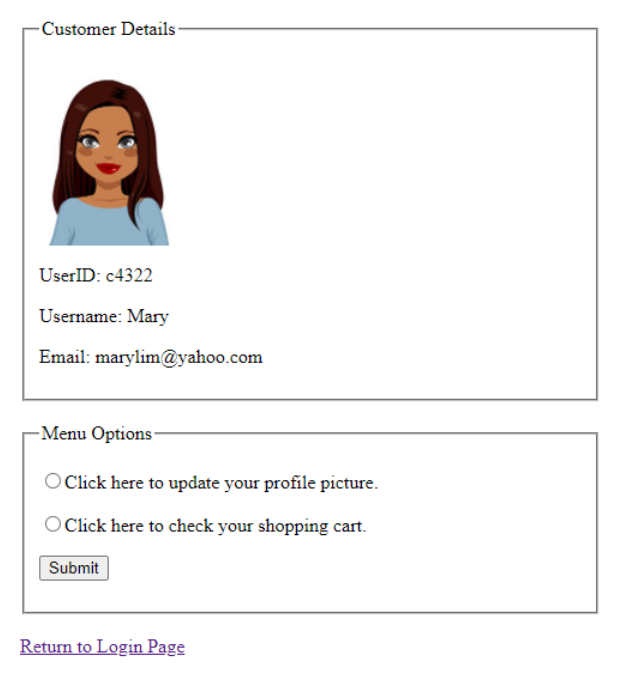
\includegraphics[scale=0.5]{C:/Users/Admin/Desktop/Github/question_bank/LyX/static/img/9569-YIJC-2021-P2-Q3-2}
\par\end{center}

\hfill{} {[}6{]}

A customer, John, does not have a profile picture and he now wishes
to upload the file \texttt{mypic.png}. This picture file will be renamed
as \texttt{John.png} before storing in the web server. 

\subsubsection*{Task 3.3 }

Write program code for the customer to select and upload a picture
file, and it should include the following: 
\begin{itemize}
\item \texttt{/menu} route in the server code to provide the customer with
a webpage \texttt{profile.html} when the option to update the profile
picture is chosen 
\item \texttt{profile.html} to allow the customer to upload a profile picture
in the \texttt{.png} format
\item \texttt{/update} route in the server code to receive the uploaded
picture file and rename it as \texttt{<username>.png} before storing
in the server\textquoteright s \texttt{\textbackslash static\textbackslash photo\textbackslash}
directory 
\item \texttt{success.html} to display a webpage informing the customer
that the profile picture has been successfully uploaded \hfill{}
{[}7{]}
\end{itemize}
The Shoppe customers usually browse through the available products
on the platform and add them to their shopping carts. When they have
decided on their purchase, they will select some or all the items
in the shopping cart before checking out to make payment. 
\noindent \begin{center}
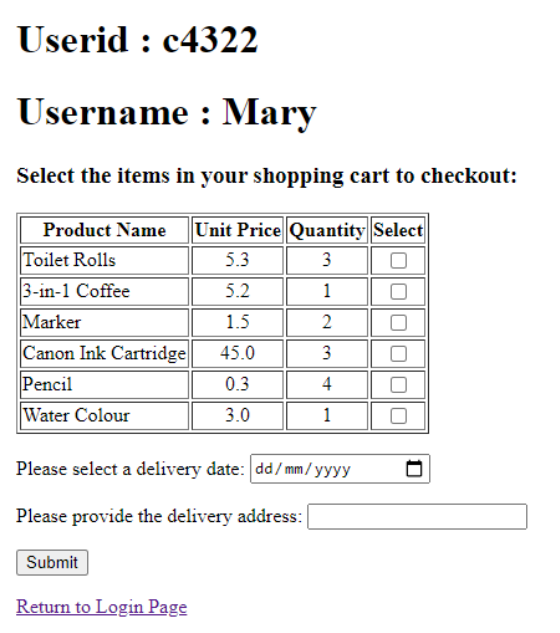
\includegraphics[scale=0.5]{C:/Users/Admin/Desktop/Github/question_bank/LyX/static/img/9569-YIJC-2021-P2-Q3-3}
\par\end{center}

\subsubsection*{Task 3.4 }

Write program code for the customer to select the items to check out
for payment, and it should include the following: 
\begin{itemize}
\item \texttt{/menu} route in the server code to query the \texttt{Cart}
table in the \texttt{shoppe.db} when the customer chooses the option
to check the shopping cart 
\item \texttt{cart.html} to display the list of items in the shopping cart
and let the customer select them for checking out; the customer will
also be required to indicate the preferred date and address for delivery 
\item \texttt{/checkout} route in the server code to receive the customer\textquoteright s
inputs and insert a record into the\texttt{ Orders} table in the\texttt{
shoppe.db }
\item \texttt{success.html} to display the \textbf{total cost} and inform
the customer that the purchase has been successfully recorded.\hfill{}
{[}14{]}
\end{itemize}